\section{Outside \sedflow Support} \label{sec:fail}
For a number of NSA galaxies, 591 out of 33,883, \sedflow~does not produce
valid posteriors
The normalizing flow of \sedflow~generates posteriors that are entirely outside
of the prior volume. 
This is driven by NSA galaxies that are outside of the support of the
\sedflow~training data. 
They lie outside of the support for two reasons: (1) some have unusually high
photometric uncertainties that are accounted for in our noise model and
(2) some have photometric colors that cannot be modeled by our SED model. 

% paragraph discussing photometric uncertainty outliers


% paragraph discussing color outliers

\begin{figure}
\begin{center}
    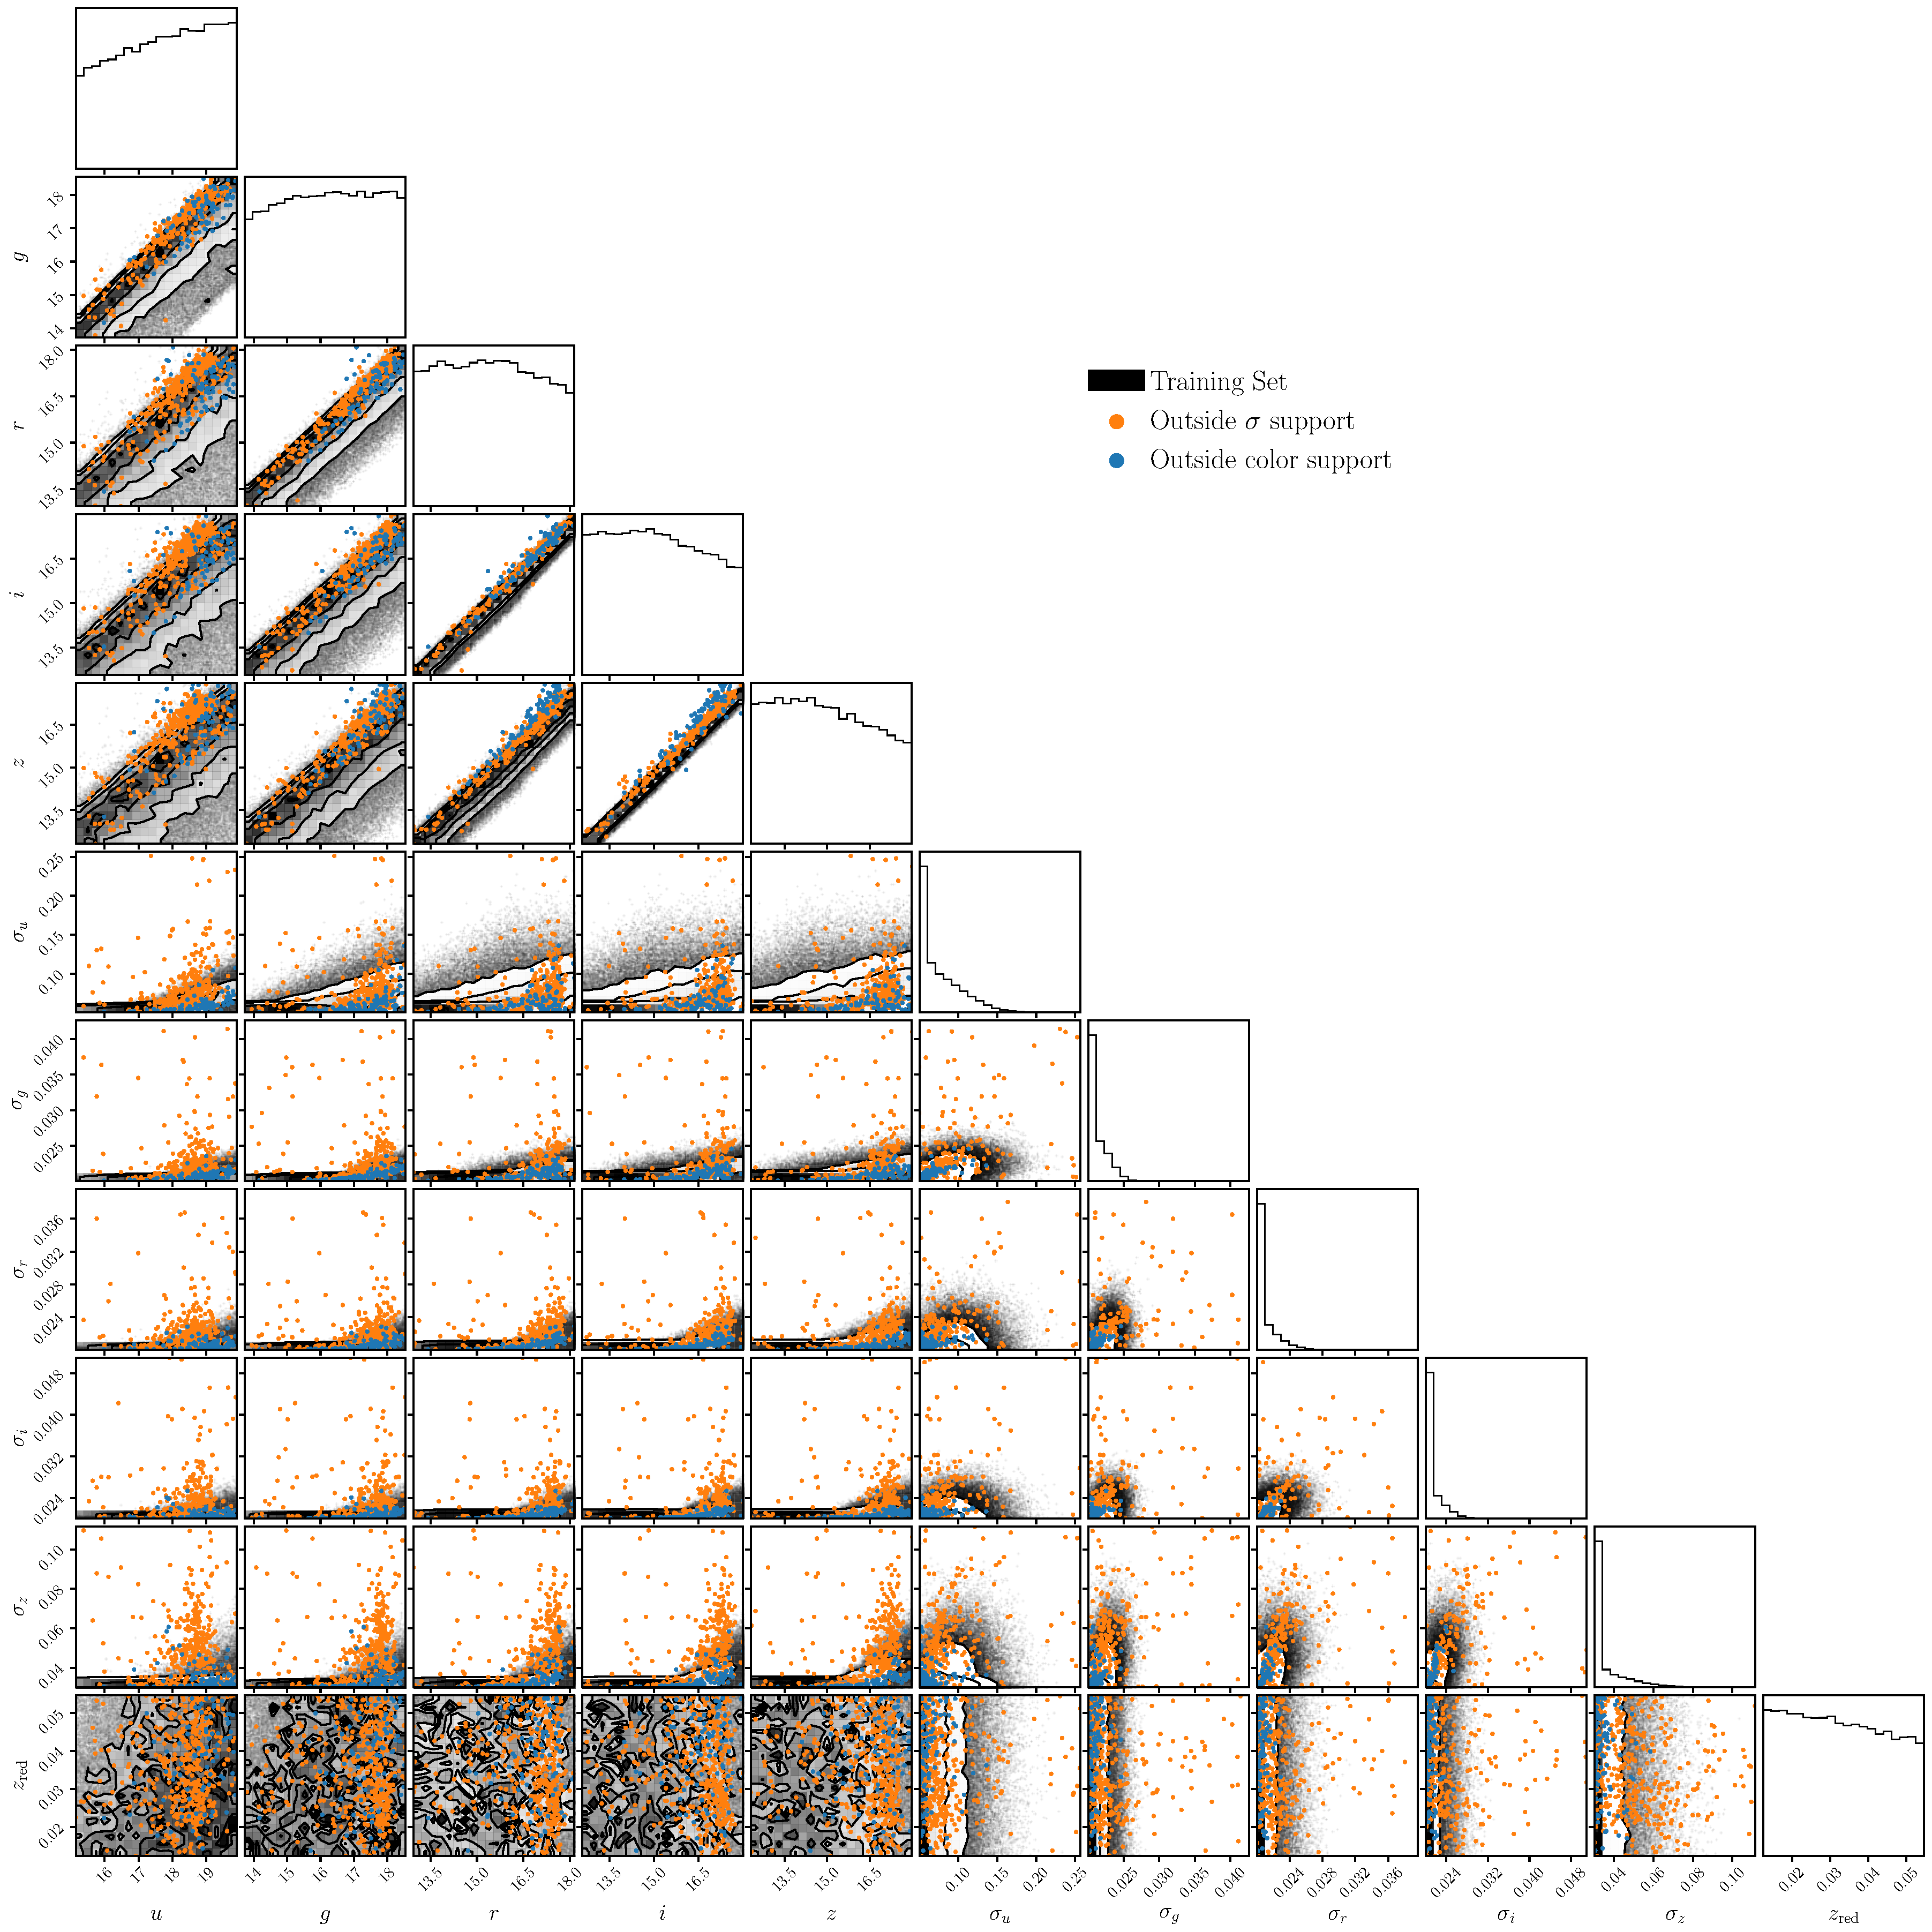
\includegraphics[width=0.9\textwidth]{figs/fails.pdf}
    \caption{\label{fig:fail}
    }
\end{center}
\end{figure}

